% Options for packages loaded elsewhere
\PassOptionsToPackage{unicode}{hyperref}
\PassOptionsToPackage{hyphens}{url}
%
\documentclass[
  ignorenonframetext,
]{beamer}
\usepackage{pgfpages}
\setbeamertemplate{caption}[numbered]
\setbeamertemplate{caption label separator}{: }
\setbeamercolor{caption name}{fg=normal text.fg}
\beamertemplatenavigationsymbolsempty
% Prevent slide breaks in the middle of a paragraph
\widowpenalties 1 10000
\raggedbottom
\setbeamertemplate{part page}{
  \centering
  \begin{beamercolorbox}[sep=16pt,center]{part title}
    \usebeamerfont{part title}\insertpart\par
  \end{beamercolorbox}
}
\setbeamertemplate{section page}{
  \centering
  \begin{beamercolorbox}[sep=12pt,center]{part title}
    \usebeamerfont{section title}\insertsection\par
  \end{beamercolorbox}
}
\setbeamertemplate{subsection page}{
  \centering
  \begin{beamercolorbox}[sep=8pt,center]{part title}
    \usebeamerfont{subsection title}\insertsubsection\par
  \end{beamercolorbox}
}
\AtBeginPart{
  \frame{\partpage}
}
\AtBeginSection{
  \ifbibliography
  \else
    \frame{\sectionpage}
  \fi
}
\AtBeginSubsection{
  \frame{\subsectionpage}
}
\usepackage{amsmath,amssymb}
\usepackage{iftex}
\ifPDFTeX
  \usepackage[T1]{fontenc}
  \usepackage[utf8]{inputenc}
  \usepackage{textcomp} % provide euro and other symbols
\else % if luatex or xetex
  \usepackage{unicode-math} % this also loads fontspec
  \defaultfontfeatures{Scale=MatchLowercase}
  \defaultfontfeatures[\rmfamily]{Ligatures=TeX,Scale=1}
\fi
\usepackage{lmodern}
\usetheme[]{Madrid}
\ifPDFTeX\else
  % xetex/luatex font selection
\fi
% Use upquote if available, for straight quotes in verbatim environments
\IfFileExists{upquote.sty}{\usepackage{upquote}}{}
\IfFileExists{microtype.sty}{% use microtype if available
  \usepackage[]{microtype}
  \UseMicrotypeSet[protrusion]{basicmath} % disable protrusion for tt fonts
}{}
\makeatletter
\@ifundefined{KOMAClassName}{% if non-KOMA class
  \IfFileExists{parskip.sty}{%
    \usepackage{parskip}
  }{% else
    \setlength{\parindent}{0pt}
    \setlength{\parskip}{6pt plus 2pt minus 1pt}}
}{% if KOMA class
  \KOMAoptions{parskip=half}}
\makeatother
\usepackage{xcolor}
\newif\ifbibliography
\usepackage{color}
\usepackage{fancyvrb}
\newcommand{\VerbBar}{|}
\newcommand{\VERB}{\Verb[commandchars=\\\{\}]}
\DefineVerbatimEnvironment{Highlighting}{Verbatim}{commandchars=\\\{\}}
% Add ',fontsize=\small' for more characters per line
\usepackage{framed}
\definecolor{shadecolor}{RGB}{248,248,248}
\newenvironment{Shaded}{\begin{snugshade}}{\end{snugshade}}
\newcommand{\AlertTok}[1]{\textcolor[rgb]{0.94,0.16,0.16}{#1}}
\newcommand{\AnnotationTok}[1]{\textcolor[rgb]{0.56,0.35,0.01}{\textbf{\textit{#1}}}}
\newcommand{\AttributeTok}[1]{\textcolor[rgb]{0.13,0.29,0.53}{#1}}
\newcommand{\BaseNTok}[1]{\textcolor[rgb]{0.00,0.00,0.81}{#1}}
\newcommand{\BuiltInTok}[1]{#1}
\newcommand{\CharTok}[1]{\textcolor[rgb]{0.31,0.60,0.02}{#1}}
\newcommand{\CommentTok}[1]{\textcolor[rgb]{0.56,0.35,0.01}{\textit{#1}}}
\newcommand{\CommentVarTok}[1]{\textcolor[rgb]{0.56,0.35,0.01}{\textbf{\textit{#1}}}}
\newcommand{\ConstantTok}[1]{\textcolor[rgb]{0.56,0.35,0.01}{#1}}
\newcommand{\ControlFlowTok}[1]{\textcolor[rgb]{0.13,0.29,0.53}{\textbf{#1}}}
\newcommand{\DataTypeTok}[1]{\textcolor[rgb]{0.13,0.29,0.53}{#1}}
\newcommand{\DecValTok}[1]{\textcolor[rgb]{0.00,0.00,0.81}{#1}}
\newcommand{\DocumentationTok}[1]{\textcolor[rgb]{0.56,0.35,0.01}{\textbf{\textit{#1}}}}
\newcommand{\ErrorTok}[1]{\textcolor[rgb]{0.64,0.00,0.00}{\textbf{#1}}}
\newcommand{\ExtensionTok}[1]{#1}
\newcommand{\FloatTok}[1]{\textcolor[rgb]{0.00,0.00,0.81}{#1}}
\newcommand{\FunctionTok}[1]{\textcolor[rgb]{0.13,0.29,0.53}{\textbf{#1}}}
\newcommand{\ImportTok}[1]{#1}
\newcommand{\InformationTok}[1]{\textcolor[rgb]{0.56,0.35,0.01}{\textbf{\textit{#1}}}}
\newcommand{\KeywordTok}[1]{\textcolor[rgb]{0.13,0.29,0.53}{\textbf{#1}}}
\newcommand{\NormalTok}[1]{#1}
\newcommand{\OperatorTok}[1]{\textcolor[rgb]{0.81,0.36,0.00}{\textbf{#1}}}
\newcommand{\OtherTok}[1]{\textcolor[rgb]{0.56,0.35,0.01}{#1}}
\newcommand{\PreprocessorTok}[1]{\textcolor[rgb]{0.56,0.35,0.01}{\textit{#1}}}
\newcommand{\RegionMarkerTok}[1]{#1}
\newcommand{\SpecialCharTok}[1]{\textcolor[rgb]{0.81,0.36,0.00}{\textbf{#1}}}
\newcommand{\SpecialStringTok}[1]{\textcolor[rgb]{0.31,0.60,0.02}{#1}}
\newcommand{\StringTok}[1]{\textcolor[rgb]{0.31,0.60,0.02}{#1}}
\newcommand{\VariableTok}[1]{\textcolor[rgb]{0.00,0.00,0.00}{#1}}
\newcommand{\VerbatimStringTok}[1]{\textcolor[rgb]{0.31,0.60,0.02}{#1}}
\newcommand{\WarningTok}[1]{\textcolor[rgb]{0.56,0.35,0.01}{\textbf{\textit{#1}}}}
\usepackage{graphicx}
\makeatletter
\def\maxwidth{\ifdim\Gin@nat@width>\linewidth\linewidth\else\Gin@nat@width\fi}
\def\maxheight{\ifdim\Gin@nat@height>\textheight\textheight\else\Gin@nat@height\fi}
\makeatother
% Scale images if necessary, so that they will not overflow the page
% margins by default, and it is still possible to overwrite the defaults
% using explicit options in \includegraphics[width, height, ...]{}
\setkeys{Gin}{width=\maxwidth,height=\maxheight,keepaspectratio}
% Set default figure placement to htbp
\makeatletter
\def\fps@figure{htbp}
\makeatother
\setlength{\emergencystretch}{3em} % prevent overfull lines
\providecommand{\tightlist}{%
  \setlength{\itemsep}{0pt}\setlength{\parskip}{0pt}}
\setcounter{secnumdepth}{-\maxdimen} % remove section numbering
\logo{
\includegraphics[height=1cm,width=3cm]{logo.png}}
\usetheme{Madrid}
\usefonttheme{serif}
\setbeamertemplate{navigation symbols}{}

\usepackage{amsmath}


\ifLuaTeX
  \usepackage{selnolig}  % disable illegal ligatures
\fi
\IfFileExists{bookmark.sty}{\usepackage{bookmark}}{\usepackage{hyperref}}
\IfFileExists{xurl.sty}{\usepackage{xurl}}{} % add URL line breaks if available
\urlstyle{same}
\hypersetup{
  pdftitle={Leksioni 3},
  pdfauthor={Endri Raco},
  hidelinks,
  pdfcreator={LaTeX via pandoc}}

\title{Leksioni 3}
\author{Endri Raco}
\date{24 April, 2024}

\begin{document}
\frame{\titlepage}

\begin{frame}[allowframebreaks]
  \tableofcontents[hideallsubsections]
\end{frame}
\hypertarget{hyrje-nuxeb-analizuxebn-e-tuxeb-dhuxebnave}{%
\section{Hyrje në Analizën e të
Dhënave}\label{hyrje-nuxeb-analizuxebn-e-tuxeb-dhuxebnave}}

\begin{frame}{Çfarë është pandas?}
\protect\hypertarget{uxe7faruxeb-uxebshtuxeb-pandas}{}
\begin{itemize}
\item
  Pandas është një bibliotekë Python që ofron një paketë të fuqishme për
  analizën e të dhënave.
\item
  Është një mjet i lehtë për t'u përdorur, por shumë i fuqishëm për
  analizën e të dhënave.
\end{itemize}
\end{frame}

\begin{frame}[fragile]{Instalimi i pandas}
\protect\hypertarget{instalimi-i-pandas}{}
\begin{Shaded}
\begin{Highlighting}[]
\NormalTok{mamba install {-}c conda{-}forge pandas}
\end{Highlighting}
\end{Shaded}
\end{frame}

\begin{frame}{Veçoritë e Pandas}
\protect\hypertarget{veuxe7orituxeb-e-pandas}{}
\begin{itemize}
\item
  Pandas është një paketë ``nivel i lartë'', që përdor shumë biblioteka
  të tjera si NumPy, matplotlib, dhe SciPy.
\item
  Një nga veçoritë më të dobishme të pandas është aftësia për të
  ndërvepruar me shumë formate të të dhënave.
\end{itemize}
\end{frame}

\begin{frame}{Formatet e të Dhënave të Mbështetura nga Pandas}
\protect\hypertarget{formatet-e-tuxeb-dhuxebnave-tuxeb-mbuxebshtetura-nga-pandas}{}
\begin{itemize}
\item
  Pandas mund të lexojë dhe shkruajë të dhëna nga shumë formate:
\item
  CSV
\item
  JSON
\item
  HTML
\item
  MS Excel
\end{itemize}
\end{frame}

\begin{frame}{Formatet e të Dhënave të Mbështetura nga Pandas}
\protect\hypertarget{formatet-e-tuxeb-dhuxebnave-tuxeb-mbuxebshtetura-nga-pandas-1}{}
\begin{itemize}
\item
  Stata
\item
  SAS
\item
  SQL (Postgresql, MySQL, Oracle, MariaDB, etj.)
\end{itemize}
\end{frame}

\begin{frame}{Strukturat e të Dhënave në Pandas}
\protect\hypertarget{strukturat-e-tuxeb-dhuxebnave-nuxeb-pandas}{}
\begin{itemize}
\tightlist
\item
  Në pandas, të dhënat në formë tabulare ruhen në objekte të tipit
  DataFrame me rreshta dhe kolona të etiketuara.
\end{itemize}

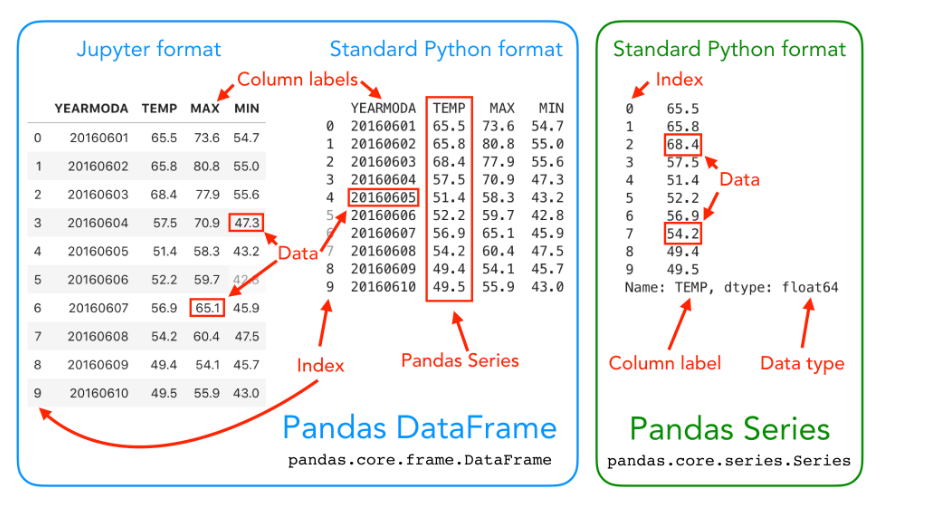
\includegraphics{./Figs/panda2.png}
\end{frame}

\begin{frame}{Strukturat Bazë të pandas në Python}
\protect\hypertarget{strukturat-bazuxeb-tuxeb-pandas-nuxeb-python}{}
\textbf{pandas DataFrame}

\begin{itemize}
\item
  \textbf{DataFrame} është një strukturë e të dhënave 2-dimensionale e
  përdorur për ruajtjen dhe manipulimin e të dhënave në formë tabelare
  (të dhëna me rreshta dhe kolona) në Python.
\item
  \textbf{DataFrame} mund të krahasohet me një spreadsheet të
  programueshëm, ku mund të ruani, organizoni dhe analizoni të dhënat me
  lehtësi.
\end{itemize}
\end{frame}

\begin{frame}{Strukturat Bazë të pandas në Python}
\protect\hypertarget{strukturat-bazuxeb-tuxeb-pandas-nuxeb-python-1}{}
\textbf{pandas Series}

\begin{itemize}
\item
  \textbf{Series} është një strukturë e të dhënave 1-dimensionale që
  përdoret për ruajtjen dhe manipulimin e një vargu vlerash.
\item
  \textbf{Series} është e ngjashme një listë, por më e zgjuar. Një
  rresht ose një kolonë në një DataFrame të pandas është në fakt një
  Series e pandas.
\end{itemize}
\end{frame}

\begin{frame}{Tiparet e Përbashkëta}
\protect\hypertarget{tiparet-e-puxebrbashkuxebta}{}
\textbf{Indekse}

\begin{itemize}
\tightlist
\item
  Të dy strukturat kanë indekse (indices) që ju lejojnë të qasni të
  dhënat lehtësisht.
\end{itemize}
\end{frame}

\begin{frame}{Strukturat e të Dhënave në Pandas}
\protect\hypertarget{strukturat-e-tuxeb-dhuxebnave-nuxeb-pandas-1}{}
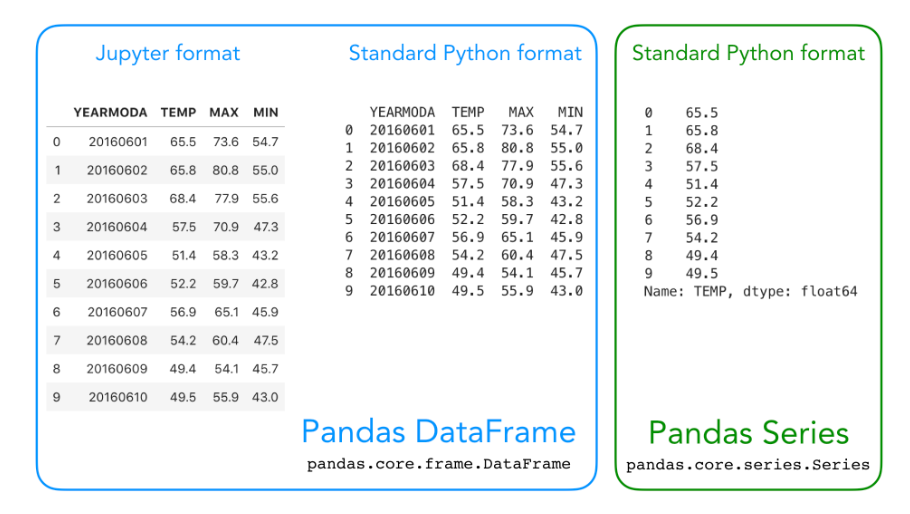
\includegraphics{./Figs/panda1.png}
\end{frame}

\begin{frame}{Leximi i të Dhënave Tabulare}
\protect\hypertarget{leximi-i-tuxeb-dhuxebnave-tabulare}{}
\begin{itemize}
\item
  Krijojmë një folder \textbf{data} në folderin tonë të punës
\item
  Shkarkojmë në folderin data skedarin nga linku:
\end{itemize}

\url{https://github.com/endri81/instatgis/blob/master/data/albania-Meteo-metadata.txt}
\end{frame}

\begin{frame}[fragile]{Leximi i të Dhënave Tabulare}
\protect\hypertarget{leximi-i-tuxeb-dhuxebnave-tabulare-1}{}
\begin{itemize}
\item
  Për të lexuar të dhënat nga një skedar CSV, përdorim funksionin
  \texttt{read\_csv()} nga pandas.
\item
  Shembull: Leximi i të dhënave nga një skedar CSV me të dhënat e motit
  nga Kumpula, Helsinki:
\end{itemize}

\begin{Shaded}
\begin{Highlighting}[]
  \ImportTok{import}\NormalTok{ pandas }\ImportTok{as}\NormalTok{ pd}
\NormalTok{  data }\OperatorTok{=}\NormalTok{ pd.read\_csv(}\StringTok{"data/albania{-}Meteo{-}metadata.txt"}\NormalTok{)}
\end{Highlighting}
\end{Shaded}
\end{frame}

\begin{frame}[fragile]{Leximi i të Dhënave Tabulare}
\protect\hypertarget{leximi-i-tuxeb-dhuxebnave-tabulare-2}{}
\begin{itemize}
\item
  Ky funksion lexon skedarin CSV dhe ruan përmbajtjen në një DataFrame
  të quajtur data.
\item
  Mund të përdorim metodën head() për të shfaqur disa nga rreshtat e
  parë të DataFrame.
\end{itemize}

\begin{Shaded}
\begin{Highlighting}[]
\NormalTok{data.head(}\DecValTok{10}\NormalTok{)  }\CommentTok{\# Kthen 10 rreshtat e parë}
\end{Highlighting}
\end{Shaded}
\end{frame}

\begin{frame}{Leximi i të Dhënave Tabulare}
\protect\hypertarget{leximi-i-tuxeb-dhuxebnave-tabulare-3}{}
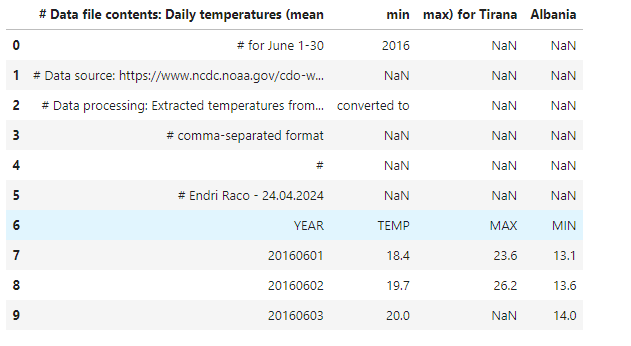
\includegraphics{./Figs/panda3.png}
\end{frame}

\begin{frame}{Analiza e të dhënave me pandas}
\protect\hypertarget{analiza-e-tuxeb-dhuxebnave-me-pandas}{}
\begin{itemize}
\item
  Gjatë analizës së një DataFrame, mund të hasim disa probleme si:

  \begin{itemize}
  \item
    \textbf{Vlerat e çuditshme}: Si NaN (``not a number''), që mund të
    tregojë një problem me leximin e skedarit.
  \item
    \textbf{Vlerat jo të pritura}: Indeksi tregon 36 rreshta, ndërsa
    duhet të ketë vetëm 30.
  \item
    \textbf{Metadata}: Rreshtat e parë përmbajnë informacione që nuk
    duam t'i procesojmë.
  \end{itemize}
\end{itemize}
\end{frame}

\begin{frame}[fragile]{Analiza e të dhënave me pandas}
\protect\hypertarget{analiza-e-tuxeb-dhuxebnave-me-pandas-1}{}
Për të zgjidhur këto probleme:

\begin{itemize}
\tightlist
\item
  Përdorni opsionin \texttt{skiprows} për të anashkaluar rreshtat me
  metadata. Për shembull, për të lexuar vetëm të dhënat relevante:
\end{itemize}

\begin{Shaded}
\begin{Highlighting}[]
\NormalTok{reg\_data }\OperatorTok{=}\NormalTok{ pd.read\_csv(}\StringTok{"data/albania{-}Meteo{-}metadata.txt"}\NormalTok{, skiprows}\OperatorTok{=}\DecValTok{8}\NormalTok{)}
\end{Highlighting}
\end{Shaded}
\end{frame}

\begin{frame}[fragile]{Analiza e të dhënave me pandas}
\protect\hypertarget{analiza-e-tuxeb-dhuxebnave-me-pandas-2}{}
\begin{itemize}
\tightlist
\item
  Kontrolloni DataFrame-in pas leximit të të dhënave. Përdorni
  funksionin \texttt{.head()} për të parë rreshtat e parë dhe
  \texttt{.tail()} për rreshtat e fundit:
\end{itemize}

\begin{Shaded}
\begin{Highlighting}[]

\NormalTok{reg\_data.head()}
\NormalTok{reg\_data.tail()}
\end{Highlighting}
\end{Shaded}
\end{frame}

\begin{frame}{Analiza e të dhënave me pandas}
\protect\hypertarget{analiza-e-tuxeb-dhuxebnave-me-pandas-3}{}
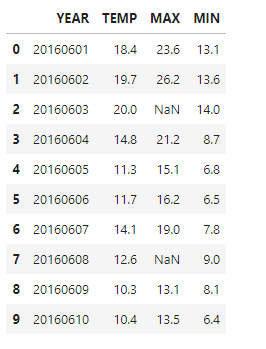
\includegraphics{./Figs/panda4.png}
\end{frame}

\begin{frame}[fragile]{Analiza e të dhënave me pandas}
\protect\hypertarget{analiza-e-tuxeb-dhuxebnave-me-pandas-4}{}
\begin{itemize}
\tightlist
\item
  Verifikoni llojin e të dhënave për të konfirmuar që është një
  DataFrame i pandas:
\end{itemize}

\begin{Shaded}
\begin{Highlighting}[]
    \BuiltInTok{type}\NormalTok{(reg\_data)}
\end{Highlighting}
\end{Shaded}
\end{frame}

\begin{frame}[fragile]{Analiza e të dhënave me pandas}
\protect\hypertarget{analiza-e-tuxeb-dhuxebnave-me-pandas-5}{}
Për të lexuar vetëm disa kolona specifike nga një skedar CSV:

\begin{itemize}
\item
  Përdorni opsionin \texttt{usecols} për të lexuar vetëm kolonat e
  dëshiruara.
\item
  Për shembull:
\end{itemize}

\begin{Shaded}
\begin{Highlighting}[]
\NormalTok{temp\_data }\OperatorTok{=}\NormalTok{ pd.read\_csv(}\StringTok{"data/albania{-}Meteo{-}metadata.txt"}\NormalTok{, skiprows}\OperatorTok{=}\DecValTok{8}\NormalTok{, usecols}\OperatorTok{=}\NormalTok{[}\StringTok{"YEAR"}\NormalTok{, }\StringTok{"TEMP"}\NormalTok{])}
\NormalTok{temp\_data.head()}
\end{Highlighting}
\end{Shaded}
\end{frame}

\begin{frame}[fragile]{Eksplorimi i DataFrame}
\protect\hypertarget{eksplorimi-i-dataframe}{}
\textbf{Hapat e parë pas ngarkimit të të dhënave}:

\begin{itemize}
\item
  Kontrolloni madhësinë e DataFrame për të kuptuar se sa rreshta dhe
  kolona përmban.
\item
  Përdorni funksionin \texttt{len()} për të marrë numrin e rreshtave:
\end{itemize}

\begin{Shaded}
\begin{Highlighting}[]
    \BuiltInTok{len}\NormalTok{(reg\_data)}
\end{Highlighting}
\end{Shaded}
\end{frame}

\begin{frame}[fragile]{Eksplorimi i DataFrame}
\protect\hypertarget{eksplorimi-i-dataframe-1}{}
\begin{itemize}
\tightlist
\item
  Përdorni atributin \texttt{shape} për të marrë një përmbledhje të
  shpejtë të madhësisë së të dhënave:
\end{itemize}

\begin{Shaded}
\begin{Highlighting}[]
\NormalTok{    reg\_data.shape}
\end{Highlighting}
\end{Shaded}

\begin{verbatim}
- Kjo tregon numrin e rreshtave dhe kolonave në DataFrame.
\end{verbatim}
\end{frame}

\begin{frame}[fragile]{Eksplorimi i DataFrame}
\protect\hypertarget{eksplorimi-i-dataframe-2}{}
\textbf{Kontrolloni emrat e kolonave}:

\begin{itemize}
\tightlist
\item
  Për të parë emrat e kolonave në DataFrame, përdorni
  \texttt{data.columns.values}:
\end{itemize}

\begin{Shaded}
\begin{Highlighting}[]
\NormalTok{    reg\_data.columns.values}
\end{Highlighting}
\end{Shaded}

\begin{itemize}
\tightlist
\item
  Kjo do të shfaqë të gjitha etiketat e kolonave.
\end{itemize}
\end{frame}

\begin{frame}[fragile]{Eksplorimi i DataFrame}
\protect\hypertarget{eksplorimi-i-dataframe-3}{}
\textbf{Indikatorët e rreshtave}:

\begin{itemize}
\tightlist
\item
  Atributi \texttt{index} tregon se si janë indeksuar rreshtat:
\end{itemize}

\begin{Shaded}
\begin{Highlighting}[]
\NormalTok{    reg\_data.index}
\end{Highlighting}
\end{Shaded}

\begin{itemize}
\tightlist
\item
  Indeksi zakonisht fillon nga 0, përfundon në 30, dhe rritet me 1. Por,
  në pandas, rreshtat mund të indeksohen edhe me karaktere ose data.
\end{itemize}
\end{frame}

\begin{frame}[fragile]{Eksplorimi i DataFrame}
\protect\hypertarget{eksplorimi-i-dataframe-4}{}
\textbf{Llojet e të dhënave për çdo kolonë}:

\begin{itemize}
\tightlist
\item
  Përdorni \texttt{data.dtypes} për të parë llojet e të dhënave në çdo
  kolonë:
\end{itemize}

\begin{Shaded}
\begin{Highlighting}[]
\NormalTok{    reg\_data.dtypes}
\end{Highlighting}
\end{Shaded}

\textbf{YEAR} është një vlerë e tipit integer (int64), ndërsa kolonat e
tjera janë float64.
\end{frame}

\begin{frame}[fragile]{Zgjedhja e Kolonave}
\protect\hypertarget{zgjedhja-e-kolonave}{}
\textbf{Sintaksa bazë për zgjedhjen e kolonave}:

\begin{itemize}
\item
  Për të zgjedhur një ose më shumë kolona nga një DataFrame, përdorni
  sintaksën \texttt{dataframe{[}value{]}}, ku \texttt{value} mund të
  jetë emri i një kolone ose një listë emrash kolonash.
\item
  Për shembull, për të zgjedhur kolonat ``YEARMODA'' dhe ``TEMP'':
\end{itemize}

\begin{Shaded}
\begin{Highlighting}[]
\NormalTok{    selection }\OperatorTok{=}\NormalTok{ reg\_data[[}\StringTok{"YEAR"}\NormalTok{, }\StringTok{"TEMP"}\NormalTok{]]}
\NormalTok{    selection}
\end{Highlighting}
\end{Shaded}
\end{frame}

\begin{frame}[fragile]{Zgjedhja e Kolonave}
\protect\hypertarget{zgjedhja-e-kolonave-1}{}
\textbf{Kontrollimi i tipit të nën-pjesës së zgjedhur}:

\begin{itemize}
\tightlist
\item
  Pasi të keni zgjedhur kolonat, mund të kontrolloni tipin e kësaj
  nën-pjesë:
\end{itemize}

\begin{Shaded}
\begin{Highlighting}[]
    \BuiltInTok{type}\NormalTok{(selection)}
\end{Highlighting}
\end{Shaded}

\begin{itemize}
\tightlist
\item
  Kjo nën-pjesë është ende një DataFrame i pandas dhe mund të përdorni
  të gjitha metodat dhe atributet e lidhura me një DataFrame.
\end{itemize}
\end{frame}

\begin{frame}[fragile]{Zgjedhja e Kolonave}
\protect\hypertarget{zgjedhja-e-kolonave-2}{}
\textbf{Kontrollimi i formës (shape) të zgjedhjes}:

\begin{itemize}
\tightlist
\item
  Për të marrë madhësinë e nën-pjesës së zgjedhur, përdorni
  \texttt{shape}:
\end{itemize}

\begin{Shaded}
\begin{Highlighting}[]
\NormalTok{    selection.shape}
\end{Highlighting}
\end{Shaded}
\end{frame}

\begin{frame}[fragile]{Zgjedhja e Kolonave}
\protect\hypertarget{zgjedhja-e-kolonave-3}{}
\textbf{Qasja e një kolone të vetme}:

\begin{itemize}
\tightlist
\item
  Për të zgjedhur një kolonë të vetme, përdorni emrin e kolonës brenda
  kllapave katrore:
\end{itemize}

\begin{Shaded}
\begin{Highlighting}[]
\NormalTok{    reg\_data[}\StringTok{"TEMP"}\NormalTok{]}
\end{Highlighting}
\end{Shaded}
\end{frame}

\begin{frame}[fragile]{Zgjedhja e Kolonave}
\protect\hypertarget{zgjedhja-e-kolonave-4}{}
\textbf{Kontrollimi i tipit të një kolone të vetme}:

\begin{itemize}
\tightlist
\item
  Për të parë tipin e një kolone të vetme, përdorni \texttt{type()}:
\end{itemize}

\begin{Shaded}
\begin{Highlighting}[]
    \BuiltInTok{type}\NormalTok{(reg\_data[}\StringTok{"TEMP"}\NormalTok{])}
\end{Highlighting}
\end{Shaded}

Çdo kolonë dhe çdo rresht në një DataFrame është në fakt një Series i
pandas, një strukturë të dhënash 1-dimensionale.
\end{frame}

\begin{frame}[fragile]{Zgjedhja e Kolonave}
\protect\hypertarget{zgjedhja-e-kolonave-5}{}
\textbf{Sintaksë alternative për zgjedhjen e kolonave}:

\begin{itemize}
\tightlist
\item
  Ju mund të përdorni një sintaksë alternative për të zgjedhur një
  kolonë:
\end{itemize}

\begin{Shaded}
\begin{Highlighting}[]
\NormalTok{    reg\_data.TEMP}
\end{Highlighting}
\end{Shaded}

\begin{itemize}
\item
  Kjo funksionon vetëm nëse emri i kolonës është një emër i vlefshëm për
  një variabël Python, dhe nuk përmban hapësira.
\item
  Sintaksa \texttt{data{[}"column"{]}} punon për çdo emër kolone, ndaj
  rekomandohet të përdorni këtë qasje.
\end{itemize}
\end{frame}

\hypertarget{statistikat-puxebrshkruese}{%
\section{Statistikat Përshkruese}\label{statistikat-puxebrshkruese}}

\begin{frame}[fragile]{Statistikat Përshkruese për DataFrame dhe Series}
\protect\hypertarget{statistikat-puxebrshkruese-puxebr-dataframe-dhe-series}{}
\textbf{Metodat e zakonshme për statistikat përshkruese}:

\begin{itemize}
\tightlist
\item
  pandas DataFrames dhe Series ofrojnë metoda për të marrë statistikat
  përshkruese, duke përfshirë \texttt{mean()}, \texttt{median()},
  \texttt{min()}, \texttt{max()}, dhe \texttt{std()} (devijimin
  standard).
\end{itemize}
\end{frame}

\begin{frame}[fragile]{Statistikat Përshkruese për DataFrame dhe Series}
\protect\hypertarget{statistikat-puxebrshkruese-puxebr-dataframe-dhe-series-1}{}
\textbf{Marrja e vlerës mesatare}:

\begin{itemize}
\tightlist
\item
  Për të kontrolluar vlerën mesatare për një kolonë të vetme (Series):
\end{itemize}

\begin{Shaded}
\begin{Highlighting}[]
\NormalTok{    reg\_data[}\StringTok{"TEMP"}\NormalTok{].mean()}
\end{Highlighting}
\end{Shaded}
\end{frame}

\begin{frame}[fragile]{Statistikat Përshkruese për DataFrame dhe Series}
\protect\hypertarget{statistikat-puxebrshkruese-puxebr-dataframe-dhe-series-2}{}
\begin{itemize}
\tightlist
\item
  Për të marrë vlerën mesatare për të gjitha kolonat në një DataFrame:
\end{itemize}

\begin{Shaded}
\begin{Highlighting}[]
\NormalTok{    reg\_data.mean()}
\end{Highlighting}
\end{Shaded}
\end{frame}

\begin{frame}[fragile]{Statistikat Përshkruese për DataFrame dhe Series}
\protect\hypertarget{statistikat-puxebrshkruese-puxebr-dataframe-dhe-series-3}{}
\textbf{Marrja e statistikave përshkruese për të gjitha kolonat}:

\begin{itemize}
\tightlist
\item
  Metoda \texttt{describe()} ofron një përmbledhje të shpejtë të
  statistikave kryesore për të gjitha atributet në DataFrame:
\end{itemize}

\begin{Shaded}
\begin{Highlighting}[]
\NormalTok{    reg\_data.describe()}
\end{Highlighting}
\end{Shaded}
\end{frame}

\hypertarget{vizualizimi-i-tuxeb-dhuxebnave-nuxeb-pandas}{%
\section{Vizualizimi i të Dhënave në
pandas}\label{vizualizimi-i-tuxeb-dhuxebnave-nuxeb-pandas}}

\begin{frame}[fragile]{Vizualizimi i të Dhënave në pandas}
\protect\hypertarget{vizualizimi-i-tuxeb-dhuxebnave-nuxeb-pandas-1}{}
\textbf{Grafikët bazë në pandas}:

\begin{itemize}
\item
  pandas ka metoda të integruara për vizualizimin e të dhënave, duke
  përdorur bibliotekën \textbf{Matplotlib}.
\item
  Për të krijuar një grafiq të thjeshtë që tregon temperaturat:
\end{itemize}

\begin{Shaded}
\begin{Highlighting}[]
\NormalTok{    reg\_data[[}\StringTok{"TEMP"}\NormalTok{, }\StringTok{"MAX"}\NormalTok{, }\StringTok{"MIN"}\NormalTok{]].plot()}
\end{Highlighting}
\end{Shaded}

\begin{itemize}
\tightlist
\item
  Ky grafik tregon të dhënat për temperatura mesatare, maksimale dhe
  minimale.
\end{itemize}
\end{frame}

\begin{frame}[fragile]{Krijimi i pandas Series nga Listat}
\protect\hypertarget{krijimi-i-pandas-series-nga-listat}{}
\textbf{Krijimi i një Series}:

\begin{itemize}
\tightlist
\item
  Ju mund të krijoni një Series nga një listë e numrave. Kjo mund të
  jetë e dobishme për të punuar me të dhënat më shpejt dhe më lehtë:
\end{itemize}

\begin{Shaded}
\begin{Highlighting}[]
\NormalTok{    number\_series }\OperatorTok{=}\NormalTok{ pd.Series([}\DecValTok{4}\NormalTok{, }\DecValTok{5}\NormalTok{, }\DecValTok{6}\NormalTok{, }\FloatTok{7.0}\NormalTok{])}
    \BuiltInTok{print}\NormalTok{(number\_series)}
\end{Highlighting}
\end{Shaded}
\end{frame}

\begin{frame}[fragile]{Krijimi i pandas Series nga Listat}
\protect\hypertarget{krijimi-i-pandas-series-nga-listat-1}{}
\begin{itemize}
\item
  pandas automatikisht konverton tipet e të dhënave, duke përdorur
  \textbf{float64} kur është e nevojshme.
\item
  Për të vendosur një indeks të personalizuar për Series:
\end{itemize}

\begin{Shaded}
\begin{Highlighting}[]
\NormalTok{    number\_series }\OperatorTok{=}\NormalTok{ pd.Series([}\DecValTok{4}\NormalTok{, }\DecValTok{5}\NormalTok{, }\DecValTok{6}\NormalTok{, }\FloatTok{7.0}\NormalTok{], index}\OperatorTok{=}\NormalTok{[}\StringTok{"a"}\NormalTok{, }\StringTok{"b"}\NormalTok{, }\StringTok{"c"}\NormalTok{, }\StringTok{"d"}\NormalTok{])}
    \BuiltInTok{print}\NormalTok{(number\_series)}
\end{Highlighting}
\end{Shaded}
\end{frame}

\begin{frame}[fragile]{Krijimi i pandas DataFrames nga Lista}
\protect\hypertarget{krijimi-i-pandas-dataframes-nga-lista}{}
\textbf{Krijimi i një DataFrame nga disa lista}:

\begin{itemize}
\tightlist
\item
  Përdorni një fjalor Python për të krijuar një DataFrame nga disa
  lista:
\end{itemize}

\begin{Shaded}
\begin{Highlighting}[]
 \CommentTok{\# Emrat e stacioneve të motit}
\NormalTok{    stacionet }\OperatorTok{=}\NormalTok{ [}\StringTok{"Tirana"}\NormalTok{, }\StringTok{"Durrës"}\NormalTok{, }\StringTok{"Shkodra"}\NormalTok{, }\StringTok{"Elbasan"}\NormalTok{]}

    \CommentTok{\# Koordinatat e gjerësisë gjeografike të stacioneve të motit}
\NormalTok{    gjeresia }\OperatorTok{=}\NormalTok{ [}\FloatTok{41.33}\NormalTok{, }\FloatTok{41.32}\NormalTok{, }\FloatTok{42.07}\NormalTok{, }\FloatTok{41.11}\NormalTok{]}

    \CommentTok{\# Koordinatat e gjatësisë gjeografike të stacioneve të motit}
\NormalTok{    gjatesia }\OperatorTok{=}\NormalTok{ [}\FloatTok{19.82}\NormalTok{, }\FloatTok{19.45}\NormalTok{, }\FloatTok{19.52}\NormalTok{, }\FloatTok{20.07}\NormalTok{]}

    \CommentTok{\# Krijimi i DataFrame nga listat}
\NormalTok{    new\_data }\OperatorTok{=}\NormalTok{ pd.DataFrame(data}\OperatorTok{=}\NormalTok{\{}\StringTok{"Emri i Stacionit"}\NormalTok{: stacionet, }\StringTok{"Gjerësia"}\NormalTok{: gjeresia, }\StringTok{"Gjatësia"}\NormalTok{: gjatesia\})}
\NormalTok{    new\_data}
\end{Highlighting}
\end{Shaded}
\end{frame}

\begin{frame}[fragile]{Krijimi i një DataFrame bosh}
\protect\hypertarget{krijimi-i-njuxeb-dataframe-bosh}{}
\textbf{Punimi me DataFrames bosh}:

\begin{itemize}
\tightlist
\item
  Ndonjëherë do të filloni me një DataFrame bosh dhe do të shtoni të
  dhënat më vonë:
\end{itemize}

\begin{Shaded}
\begin{Highlighting}[]
\NormalTok{    df }\OperatorTok{=}\NormalTok{ pd.DataFrame()}
    \BuiltInTok{print}\NormalTok{(df)}
\end{Highlighting}
\end{Shaded}
\end{frame}

\hypertarget{manipulimi-i-tuxeb-dhuxebnave}{%
\section{Manipulimi i të dhënave}\label{manipulimi-i-tuxeb-dhuxebnave}}

\begin{frame}[fragile]{Krijimi i Kolonave të Reja në DataFrame}
\protect\hypertarget{krijimi-i-kolonave-tuxeb-reja-nuxeb-dataframe}{}
\textbf{Krijimi i kolonave të reja}:

\begin{itemize}
\item
  Një nga gjërat më të zakonshme për të bërë në pandas është krijimi i
  kolonave të reja bazuar në kalkulime midis kolonave të ndryshme.
\item
  Për të krijuar një kolonë të re, thjesht specifikoni emrin e kolonës
  dhe caktoni një vlerë të paracaktuar.
\item
  Për shembull, për të krijuar një kolonë ``DIFF'' me vlerën 0.0:
\end{itemize}

\begin{Shaded}
\begin{Highlighting}[]
\NormalTok{    reg\_data[}\StringTok{"DIFF"}\NormalTok{] }\OperatorTok{=} \FloatTok{0.0}
\end{Highlighting}
\end{Shaded}
\end{frame}

\begin{frame}[fragile]{Krijimi i Kolonave të Reja në DataFrame}
\protect\hypertarget{krijimi-i-kolonave-tuxeb-reja-nuxeb-dataframe-1}{}
\textbf{Kontrollimi i tipit të të dhënave për kolonën e re}:

\begin{itemize}
\tightlist
\item
  Mund të kontrolloni tipin e të dhënave të kolonës së re për të
  konfirmuar që pandas e ka njohur si float:
\end{itemize}

\begin{Shaded}
\begin{Highlighting}[]
\NormalTok{    reg\_data[}\StringTok{"DIFF"}\NormalTok{].dtypes}
\end{Highlighting}
\end{Shaded}
\end{frame}

\begin{frame}[fragile]{Përditësimi i kolonës ``DIFF'' me kalkulime}
\protect\hypertarget{puxebrdituxebsimi-i-kolonuxebs-diff-me-kalkulime}{}
\textbf{Përditësimi i kolonës ``DIFF'' me kalkulime}:

\begin{itemize}
\tightlist
\item
  Për të llogaritur diferencën midis kolonave ``MAX'' dhe ``MIN'', mund
  të përdorni një operacion matematikor dhe të përditësoni kolonën
  ``DIFF'':
\end{itemize}

\begin{Shaded}
\begin{Highlighting}[]
\NormalTok{    reg\_data[}\StringTok{"DIFF"}\NormalTok{] }\OperatorTok{=}\NormalTok{ reg\_data[}\StringTok{"MAX"}\NormalTok{] }\OperatorTok{{-}}\NormalTok{ reg\_data[}\StringTok{"MIN"}\NormalTok{]}
\NormalTok{    reg\_data.head()}
\end{Highlighting}
\end{Shaded}
\end{frame}

\begin{frame}[fragile]{Krijimi i një kolone për të kthyer Celsius në
Fahrenheit}
\protect\hypertarget{krijimi-i-njuxeb-kolone-puxebr-tuxeb-kthyer-celsius-nuxeb-fahrenheit}{}
\textbf{Krijimi i një kolone për të kthyer Celsius në Fahrenheit}:

\begin{itemize}
\tightlist
\item
  Për të kthyer vlerat nga Celsius në Fahrenheit dhe t'i ruani në një
  kolonë të re, mund të përdorni formulën \(F = (C \times 9/5) + 32\):
\end{itemize}

\begin{Shaded}
\begin{Highlighting}[]
\NormalTok{    reg\_data[}\StringTok{"TEMP\_FAHRENHEIT"}\NormalTok{] }\OperatorTok{=}\NormalTok{ (reg\_data[}\StringTok{"TEMP"}\NormalTok{] }\OperatorTok{*}\NormalTok{ (}\DecValTok{9}\OperatorTok{/}\DecValTok{5}\NormalTok{)) }\OperatorTok{+} \DecValTok{32}
\NormalTok{    reg\_data.head()}
\end{Highlighting}
\end{Shaded}
\end{frame}

\hypertarget{zgjedhja-e-rreshtave-dhe-shtyllave}{%
\section{Zgjedhja e rreshtave dhe
shtyllave}\label{zgjedhja-e-rreshtave-dhe-shtyllave}}

\begin{frame}{Zgjedhja e rreshtave dhe shtyllave}
\protect\hypertarget{zgjedhja-e-rreshtave-dhe-shtyllave-1}{}
\begin{itemize}
\item
  Shpesh të zgjidhni rreshta dhe kolona të veçanta në një DataFrame
  pandas.
\item
  Këtu janë disa mënyra të ndryshme për të zgjedhur nënsete të një
  DataFrame, të shpjeguara me shembuj dhe në formatin R Markdown.
\end{itemize}
\end{frame}

\begin{frame}[fragile]{Zgjedhja e disa rreshtave:}
\protect\hypertarget{zgjedhja-e-disa-rreshtave}{}
\begin{itemize}
\item
  Për të zgjedhur një nëngrup të veçantë të rreshtave nga një DataFrame,
  mund të përdorni indeksimin për të marrë pjesë të DataFrame.
\item
  Këtu është një shembull që zgjedh pesë rreshtat e parë dhe i ruan në
  një variabël të quajtur selection:
\end{itemize}

\begin{Shaded}
\begin{Highlighting}[]
\NormalTok{selection }\OperatorTok{=}\NormalTok{ reg\_data.iloc[}\DecValTok{0}\NormalTok{:}\DecValTok{5}\NormalTok{]  }\CommentTok{\# Zgjidhni pesë rreshtat e parë}
\NormalTok{selection  }\CommentTok{\# shfaq përzgjedhjen}
\end{Highlighting}
\end{Shaded}

\begin{itemize}
\tightlist
\item
  Në këtë rast, kemi zgjedhur pesë rreshtat e parë (indekset 0-4) duke
  përdorur indeksimin e thjeshtë.
\end{itemize}
\end{frame}

\begin{frame}[fragile]{Zgjedhja e disa rreshtave dhe kolonave}
\protect\hypertarget{zgjedhja-e-disa-rreshtave-dhe-kolonave}{}
\begin{itemize}
\item
  Për të zgjedhur një subset të rreshtave dhe kolonave, mund të përdorni
  \textbf{loc} që zgjedh të dhënat bazuar në emrat e kolonave dhe
  rreshtave.
\item
  Këtu është një shembull që zgjedh vlerat e kolonës ``TEMP'' nga
  rreshtat 0-5:
\end{itemize}

\begin{Shaded}
\begin{Highlighting}[]
\NormalTok{selection }\OperatorTok{=}\NormalTok{ reg\_data.loc[}\DecValTok{0}\NormalTok{:}\DecValTok{5}\NormalTok{, }\StringTok{"TEMP"}\NormalTok{]}
\NormalTok{selection}
\end{Highlighting}
\end{Shaded}

\begin{itemize}
\tightlist
\item
  Në këtë rast, marrim gjashtë rreshtat e parë (indekset 0-5) duke
  përdorur emrat e rreshtave.
\end{itemize}
\end{frame}

\begin{frame}[fragile]{Zgjedhja e shumëfishtë e kolonave me loc:}
\protect\hypertarget{zgjedhja-e-shumuxebfishtuxeb-e-kolonave-me-loc}{}
\begin{itemize}
\item
  Mund të zgjidhni më shumë se një kolonë duke përdorur loc me një listë
  kolonash.
\item
  Këtu është një shembull që zgjedh kolonat ``TEMP'' dhe
  ``TEMP\_FAHRENHEIT'' nga rreshtat 0-5:
\end{itemize}

\begin{Shaded}
\begin{Highlighting}[]
\CommentTok{\# Përdorim të saktë të loc me lista të kolonave}
\NormalTok{selection }\OperatorTok{=}\NormalTok{ reg\_data.loc[}\DecValTok{0}\NormalTok{:}\DecValTok{5}\NormalTok{, [}\StringTok{"TEMP"}\NormalTok{, }\StringTok{"TEMP\_FAHRENHEIT"}\NormalTok{]]  }\CommentTok{\# Zgjedh pesë rreshtat e parë dhe dy kolon}
\NormalTok{selection}
\end{Highlighting}
\end{Shaded}
\end{frame}

\begin{frame}[fragile]{Zgjedhja e një rreshti të vetëm}
\protect\hypertarget{zgjedhja-e-njuxeb-rreshti-tuxeb-vetuxebm}{}
\begin{itemize}
\item
  Mund të zgjidhni gjithashtu një rresht të vetëm nga një pozicion i
  caktuar duke përdorur indeksimin \texttt{.loc{[}{]}}.
\item
  Këtu zgjedhim të gjitha vlerat e të dhënave duke përdorur indeksin 4
  (rreshti i 5-të):
\item
  Zgjidhni një rresht duke përdorur indeksin
\end{itemize}

\begin{Shaded}
\begin{Highlighting}[]
\CommentTok{\# Select one row using index}
\NormalTok{row }\OperatorTok{=}\NormalTok{ reg\_data.loc[}\DecValTok{4}\NormalTok{]}
\NormalTok{row}
\end{Highlighting}
\end{Shaded}
\end{frame}

\begin{frame}[fragile]{Zgjedhja e një rreshti të vetëm}
\protect\hypertarget{zgjedhja-e-njuxeb-rreshti-tuxeb-vetuxebm-1}{}
\begin{itemize}
\item
  Indeksimi \texttt{.loc{[}{]}} kthen vlerat nga ajo pozicion si një
  pd.Series ku indekset në fakt janë emrat e kolonave të atyre
  variablave.
\item
  Prandaj, mund të hyni në vlerën e një kolone të veçantë duke u
  referuar në indeksin e saj duke përdorur formatin e mëposhtëm (të dy
  duhet të funksionojnë):
\end{itemize}
\end{frame}

\begin{frame}[fragile]{Zgjedhja e një rreshti të vetëm}
\protect\hypertarget{zgjedhja-e-njuxeb-rreshti-tuxeb-vetuxebm-2}{}
\begin{itemize}
\tightlist
\item
  Printoni një atribut nga rreshti i zgjedhur
\end{itemize}

\begin{Shaded}
\begin{Highlighting}[]
\NormalTok{row[}\StringTok{"TEMP"}\NormalTok{]}
\end{Highlighting}
\end{Shaded}
\end{frame}

\begin{frame}[fragile]{Zgjedhja e një vlere të vetme bazuar në rresht
dhe kolonë}
\protect\hypertarget{zgjedhja-e-njuxeb-vlere-tuxeb-vetme-bazuar-nuxeb-rresht-dhe-kolonuxeb}{}
\begin{itemize}
\item
  Në disa raste është mjaftueshëm të hysh në një vlerë të vetme në një
  DataFrame.
\item
  Në këtë rast, mund të përdorim \texttt{DataFrame.at} në vend të
  \texttt{Data.Frame.loc}.
\end{itemize}
\end{frame}

\begin{frame}[fragile]{Zgjedhja e një vlere të vetme bazuar në rresht
dhe kolonë}
\protect\hypertarget{zgjedhja-e-njuxeb-vlere-tuxeb-vetme-bazuar-nuxeb-rresht-dhe-kolonuxeb-1}{}
\begin{itemize}
\tightlist
\item
  Zgjidhni temperaturën (kolonën TEMP) në rreshtin e parë (indeksi 0) të
  DataFrame tonë.
\end{itemize}

\begin{Shaded}
\begin{Highlighting}[]
\NormalTok{reg\_data.at[}\DecValTok{0}\NormalTok{, }\StringTok{"TEMP"}\NormalTok{]}
\end{Highlighting}
\end{Shaded}
\end{frame}

\begin{frame}[fragile]{Zgjedhjet nga pozicioni integer (opsionale)}
\protect\hypertarget{zgjedhjet-nga-pozicioni-integer-opsionale}{}
\begin{itemize}
\item
  \texttt{.loc} dhe \texttt{.at} bazohen në \emph{etiketat e aksit},
  emrat e kolonave dhe rreshtave.
\item
  Etiketat e aksit mund të jenë gjëra të tjera përveç vlerave
  ``tradicionale'' të indeksit (p.sh., \texttt{0}, \texttt{1}, \ldots).
\item
  Për shembull, datat kohore shpesh përdoren si indeksi i rreshtave për
  rreshtat e listuara sipas dates dhe kohës së të dhënave.
\end{itemize}
\end{frame}

\begin{frame}[fragile]{Zgjedhjet nga pozicioni integer (opsionale)}
\protect\hypertarget{zgjedhjet-nga-pozicioni-integer-opsionale-1}{}
\begin{itemize}
\item
  \texttt{.iloc} është një operator tjetër indeksimi që bazohet në
  \emph{vlerat e integer} indeksit.
\item
  Duke përdorur \texttt{.iloc}, është e mundur të referohemi gjithashtu
  në kolonat bazuar në vlerën e tyre të indeksit.
\item
  Për shembull, \texttt{reg\_data.iloc{[}0,0{]}} do të kthejë
  \texttt{20160601} në DataFrame-in tonë shembull.
\end{itemize}
\end{frame}

\begin{frame}[fragile]{Zgjedhjet nga pozicioni integer (opsionale)}
\protect\hypertarget{zgjedhjet-nga-pozicioni-integer-opsionale-2}{}
\begin{itemize}
\tightlist
\item
  Për shembull, mund të zgjidhni nga një grup rreshtash tek kolonat YEAR
  dhe TEMP bazuar në indeksin e tyre.
\end{itemize}

\begin{Shaded}
\begin{Highlighting}[]
\NormalTok{reg\_data.iloc[}\DecValTok{0}\NormalTok{:}\DecValTok{5}\NormalTok{:, }\DecValTok{0}\NormalTok{:}\DecValTok{2}\NormalTok{]}
\end{Highlighting}
\end{Shaded}
\end{frame}

\begin{frame}[fragile]{Zgjedhjet nga pozicioni integer (opsionale)}
\protect\hypertarget{zgjedhjet-nga-pozicioni-integer-opsionale-3}{}
\begin{itemize}
\tightlist
\item
  Për të aksesuar vlerën në rreshtin e parë dhe kolonën e dytë (TEMP),
  sintaksa për iloc do të ishte:
\end{itemize}

\begin{Shaded}
\begin{Highlighting}[]
\NormalTok{reg\_data.iloc[}\DecValTok{0}\NormalTok{, }\DecValTok{1}\NormalTok{]}
\end{Highlighting}
\end{Shaded}
\end{frame}

\begin{frame}[fragile]{Zgjedhjet nga pozicioni integer (opsionale)}
\protect\hypertarget{zgjedhjet-nga-pozicioni-integer-opsionale-4}{}
\begin{itemize}
\item
  Gjithashtu mund të qaseni në rreshta individuale duke përdorur iloc.
\item
  Le të shohim rreshtin e fundit të të dhënave:
\end{itemize}

\begin{Shaded}
\begin{Highlighting}[]
\NormalTok{reg\_data.iloc[}\OperatorTok{{-}}\DecValTok{1}\NormalTok{]}
\end{Highlighting}
\end{Shaded}
\end{frame}

\hypertarget{filtrimi-dhe-puxebrdituxebsimi-i-tuxeb-dhuxebnave}{%
\section{Filtrimi dhe përditësimi i të
dhënave}\label{filtrimi-dhe-puxebrdituxebsimi-i-tuxeb-dhuxebnave}}

\begin{frame}[fragile]{Filtrimi dhe përditësimi i të dhënave}
\protect\hypertarget{filtrimi-dhe-puxebrdituxebsimi-i-tuxeb-dhuxebnave-1}{}
\begin{itemize}
\item
  Një veçori shumë e dobishme në pandas është aftësia për të filtruar
  dhe zgjedhur rreshtat në bazë të një deklarate me kusht.
\item
  Në vijim është një shembull se si të zgjidhni rreshtat kur temperatura
  në Celsius ka qenë më e lartë se 15 gradë dhe t'i ruani ato në
  variabël \textbf{temp\_ngroht} (temperature të ngrohta).
\item
  pandas kontrollon nëse kushti është i vërtetë ose fals për çdo rresht,
  dhe kthen ato rreshta ku kushti është i vërtetë:
\end{itemize}

\begin{Shaded}
\begin{Highlighting}[]
\CommentTok{\# Kontrollo kushtin}
\NormalTok{reg\_data[}\StringTok{"TEMP"}\NormalTok{] }\OperatorTok{\textgreater{}} \DecValTok{15}
\CommentTok{\# Zgjidh rreshtat me temperaturë Celsius më të lartë se 15 gradë}
\NormalTok{temp\_ngroht }\OperatorTok{=}\NormalTok{ reg\_data.loc[reg\_data[}\StringTok{"TEMP"}\NormalTok{] }\OperatorTok{\textgreater{}} \DecValTok{15}\NormalTok{]}
\NormalTok{temp\_ngroht}
\end{Highlighting}
\end{Shaded}
\end{frame}

\begin{frame}{Filtrimi dhe përditësimi i të dhënave}
\protect\hypertarget{filtrimi-dhe-puxebrdituxebsimi-i-tuxeb-dhuxebnave-2}{}
\begin{itemize}
\item
  Është gjithashtu e mundur të kombinoni disa kritere njëkohësisht.
\item
  Këtu, zgjedhim temperaturat mbi 15 gradë që u regjistruan në gjysmën e
  dytë të qershorit në vitin 2016 (pra. YEAR \textgreater= 20160615).
\item
  Kombinimi i kritereve të shumta mund të bëhet me operatorin \& (DHE)
  ose operatorin \textbar{} (OSE).
\item
  Është shpesh e dobishme të ndani kushtet e ndryshme duke përdorur
  paranteza ().
\end{itemize}
\end{frame}

\begin{frame}[fragile]{Filtrimi dhe përditësimi i të dhënave}
\protect\hypertarget{filtrimi-dhe-puxebrdituxebsimi-i-tuxeb-dhuxebnave-3}{}
\begin{Shaded}
\begin{Highlighting}[]
\CommentTok{\# Zgjidh rreshtat me temperaturë Celsius më të lartë se 15 gradë nga fundi i qershorit 2016}
\NormalTok{temp\_ngroht }\OperatorTok{=}\NormalTok{ reg\_data.loc[(reg\_data[}\StringTok{"TEMP"}\NormalTok{] }\OperatorTok{\textgreater{}} \DecValTok{15}\NormalTok{) }\OperatorTok{\&}\NormalTok{ (reg\_data[}\StringTok{"YEAR"}\NormalTok{] }\OperatorTok{\textgreater{}=} \DecValTok{20160615}\NormalTok{)]}
\NormalTok{temp\_ngroht}
\end{Highlighting}
\end{Shaded}

\begin{itemize}
\tightlist
\item
  Tani kemi një nën-set të DataFrame tonë me vetëm rreshtat ku TEMP
  është mbi 15 dhe datat në kolonën YEAR fillojnë nga 15 qershori.
\end{itemize}
\end{frame}

\begin{frame}{Filtrimi dhe përditësimi i të dhënave}
\protect\hypertarget{filtrimi-dhe-puxebrdituxebsimi-i-tuxeb-dhuxebnave-4}{}
\begin{itemize}
\item
  Vini re se vlerat e indeksit (numrat në të majtë) tregojnë ende
  pozicionet nga DataFrame origjinale.
\item
  Është e mundur të rivendosni indeksin duke përdorur funksionin
  \textbf{reset\_index()}, i cili mund të jetë i dobishëm në disa raste
  për të qenë në gjendje të shkëputni të dhënat në një mënyrë të
  ngjashme me atë më lart.
\end{itemize}
\end{frame}

\begin{frame}{Filtrimi dhe përditësimi i të dhënave}
\protect\hypertarget{filtrimi-dhe-puxebrdituxebsimi-i-tuxeb-dhuxebnave-5}{}
\begin{itemize}
\item
  Në mënyrë parazgjedhëse \textbf{reset\_index()} do të krijojë një
  kolonë të re quajtur \textbf{index} për të mbajtur gjurmën e indeksit
  të mëparshëm, që mund të jetë e dobishme në disa raste.
\item
  Ky nuk është rasti këtu, kështu që mund ta injorojmë këtë veprim duke
  kaluar parametrin drop=True.
\end{itemize}
\end{frame}

\begin{frame}[fragile]{Filtrimi dhe përditësimi i të dhënave}
\protect\hypertarget{filtrimi-dhe-puxebrdituxebsimi-i-tuxeb-dhuxebnave-6}{}
\begin{Shaded}
\begin{Highlighting}[]
\CommentTok{\# Rivendos indeksin}
\NormalTok{temp\_ngroht }\OperatorTok{=}\NormalTok{ temp\_ngroht.reset\_index(drop}\OperatorTok{=}\VariableTok{True}\NormalTok{)}
\NormalTok{temp\_ngroht}
\end{Highlighting}
\end{Shaded}

Siç mund të shihni, tani vlerat e indeksit shkojnë nga 0 në 12 tani.
\end{frame}

\hypertarget{vlerat-quxeb-mungojnuxeb-missing-values}{%
\section{Vlerat që mungojnë (Missing
values)}\label{vlerat-quxeb-mungojnuxeb-missing-values}}

\begin{frame}{Vlerat që mungojnë (Missing values)}
\protect\hypertarget{vlerat-quxeb-mungojnuxeb-missing-values-1}{}
\begin{itemize}
\item
  Siç mund të keni vënë re deri më tani, kemi disa vlera të humbura në
  kolonat e temperaturës minimale, maksimale, dhe diferencës (MIN, MAX,
  dhe DIFF).
\item
  Këto vlera të humbura shënohen si \textbf{NaN} (jo një numër).
\end{itemize}
\end{frame}

\begin{frame}{Vlerat që mungojnë (Missing values)}
\protect\hypertarget{vlerat-quxeb-mungojnuxeb-missing-values-2}{}
\begin{itemize}
\item
  Të dhënat e munguara në tabelë është një situatë e zakonshme dhe
  zakonisht duam t'i trajtojmë ato
\item
  Procedurat e zakonshme për të trajtuar vlerat NaN janë ose t'i largoni
  ato nga DataFrame ose t'i mbushni ato me një vlerë tjetër.
\item
  Në pandas të dyja këto opsione janë të lehta për tu bërë.
\end{itemize}
\end{frame}

\begin{frame}{Vlerat që mungojnë (Missing values)}
\protect\hypertarget{vlerat-quxeb-mungojnuxeb-missing-values-3}{}
\begin{itemize}
\item
  Le të shohim së pari si mund të largojmë vlerat e munguara (pra, të
  pastroni të dhënat) duke përdorur funksionin \textbf{.dropna()}.
\item
  Brenda funksionit mund të kaloni një listë të kolonave nga të cilat
  vlerat duhet të gjeni NaN duke përdorur parametrin subset.
\item
  Outputi do të heqë çdo rresht që përmban vlera NaN nga grupi i
  kolonave të dhëna në parametrin subset.
\end{itemize}
\end{frame}

\begin{frame}[fragile]{Vlerat që mungojnë (Missing values)}
\protect\hypertarget{vlerat-quxeb-mungojnuxeb-missing-values-4}{}
\begin{Shaded}
\begin{Highlighting}[]
\CommentTok{\# Largo vlerat NaN bazuar në kolonën MIN}
\NormalTok{    temp\_ngroht\_clean }\OperatorTok{=}\NormalTok{ temp\_ngroht.dropna(subset}\OperatorTok{=}\NormalTok{[}\StringTok{"MIN"}\NormalTok{])}
\NormalTok{    temp\_ngroht\_clean}
\end{Highlighting}
\end{Shaded}

Siç mund të shihni nga tabela e mësipërme (dhe ndryshimi në vlerat e
indeksit), tani kemi një DataFrame pa vlerat NaN.
\end{frame}

\begin{frame}[fragile]{Vlerat që mungojnë (Missing values)}
\protect\hypertarget{vlerat-quxeb-mungojnuxeb-missing-values-5}{}
\begin{itemize}
\item
  Vini re se zëvendësuam variablin fillestare `temp\_ngroht' me
  versionin ku nuk ka të dhëna missing.
\item
  Funksioni \texttt{.dropna()} mund të aplikohet edhe ``inplace'' që do
  të thotë që funksioni përditëson objektin DataFrame dhe kthen
  \texttt{None}:
\end{itemize}

\begin{Shaded}
\begin{Highlighting}[]
\NormalTok{    temp\_ngroht.dropna(subset}\OperatorTok{=}\NormalTok{[}\StringTok{\textquotesingle{}MIN\textquotesingle{}}\NormalTok{], inplace}\OperatorTok{=}\VariableTok{True}\NormalTok{)}
\end{Highlighting}
\end{Shaded}
\end{frame}

\begin{frame}{Vlerat që mungojnë (Missing values)}
\protect\hypertarget{vlerat-quxeb-mungojnuxeb-missing-values-6}{}
\begin{itemize}
\item
  Një opsion tjetër është të mbushni vlerat e munguara me një vlerë duke
  përdorur funksionin \textbf{fillna()}.
\item
  Këtu mund të mbushni vlerat e munguara me vlerën -9999.
\item
  Vini re që këtë herë nuk i jepni parametrin subset.
\end{itemize}
\end{frame}

\begin{frame}[fragile]{Vlerat që mungojnë (Missing values)}
\protect\hypertarget{vlerat-quxeb-mungojnuxeb-missing-values-7}{}
\begin{Shaded}
\begin{Highlighting}[]
\CommentTok{\# Mbush vlerat NaN}
\NormalTok{fill\_data }\OperatorTok{=}\NormalTok{ reg\_data.fillna(}\OperatorTok{{-}}\DecValTok{9999}\NormalTok{)}
\NormalTok{fill\_data.head(}\DecValTok{5}\NormalTok{)}
\end{Highlighting}
\end{Shaded}

Si rezultat tani kemi një DataFrame ku vlerat e munguara janë mbushur me
vlerën -9999.
\end{frame}

\begin{frame}{Vlerat që mungojnë (Missing values)}
\protect\hypertarget{vlerat-quxeb-mungojnuxeb-missing-values-8}{}
\begin{itemize}
\item
  Në shumë raste, mbushja e të dhënave me një vlerë specifike është e
  rrezikshme sepse ju përfundoni duke ndryshuar të dhënat reale, e cila
  mund të ndikojë në rezultatet e analizës suaj.
\item
  Për shembull, në rastin e mësipërm do të kishim ndryshuar dramatikisht
  kolonat e diferencës së temperaturës sepse vlerat -9999 nuk janë një
  diferencë temperaturash aktuale!
\end{itemize}
\end{frame}

\hypertarget{konvertimi-i-tipit-tuxeb-tuxeb-dhuxebnave}{%
\section{Konvertimi i tipit të të
dhënave}\label{konvertimi-i-tipit-tuxeb-tuxeb-dhuxebnave}}

\begin{frame}{Konvertimi i tipit të të dhënave}
\protect\hypertarget{konvertimi-i-tipit-tuxeb-tuxeb-dhuxebnave-1}{}
\begin{itemize}
\item
  Ka raste kur do të duhet të kthejmë të dhënat e ruajtura brenda një
  Series në një lloj tjetër të të dhënave, për shembull, nga float në
  integer.
\item
  Kujtoni, që kemi bërë konvertimin e llojeve të të dhënave duke
  përdorur funksionet e ndërtuara në Python si int() ose str().
\item
  Për vlerat në pandas DataFrames dhe Series, mund të përdorim metodën
  astype().
\end{itemize}
\end{frame}

\begin{frame}{Konvertimi i tipit të të dhënave}
\protect\hypertarget{konvertimi-i-tipit-tuxeb-tuxeb-dhuxebnave-2}{}
\textbf{Kujdes me konvertimet nga float në integer.}

\begin{itemize}
\item
  Konvertimi thjesht heq pjesën pas presjes dhjetore, kështu që të
  gjitha vlerat janë rrumbullakosur poshtë në numrin e plotë më të
  afërt.
\item
  Për shembull, 99.99 do të shkurtohet në 99 si një integer, kur duhet
  të rrumbullohet lart në 100.
\end{itemize}
\end{frame}

\begin{frame}[fragile]{Konvertimi i tipit të të dhënave}
\protect\hypertarget{konvertimi-i-tipit-tuxeb-tuxeb-dhuxebnave-3}{}
\begin{itemize}
\tightlist
\item
  Lidhja e funksioneve \textbf{round} dhe konvertimi i tipeve e zgjidh
  këtë situatë, pasi komanda \texttt{.round(0).astype(int)} fillimisht
  rrumbullon vlerat me zero presje dhe pastaj i konverton ato në
  integer.
\end{itemize}
\end{frame}

\begin{frame}[fragile]{Konvertimi i tipit të të dhënave}
\protect\hypertarget{konvertimi-i-tipit-tuxeb-tuxeb-dhuxebnave-4}{}
\begin{Shaded}
\begin{Highlighting}[]
\BuiltInTok{print}\NormalTok{(}\StringTok{"Vlerat origjinale:"}\NormalTok{)}
\NormalTok{reg\_data[}\StringTok{"TEMP"}\NormalTok{].head()}
\end{Highlighting}
\end{Shaded}

\begin{Shaded}
\begin{Highlighting}[]
\BuiltInTok{print}\NormalTok{(}\StringTok{"Vlerat e shkurtra në integer:"}\NormalTok{)}
\NormalTok{reg\_data[}\StringTok{"TEMP"}\NormalTok{].astype(}\BuiltInTok{int}\NormalTok{).head()}
\end{Highlighting}
\end{Shaded}

\begin{Shaded}
\begin{Highlighting}[]
\BuiltInTok{print}\NormalTok{(}\StringTok{"Vlerat e rrumbulluara në integer:"}\NormalTok{)}
\NormalTok{reg\_data[}\StringTok{"TEMP"}\NormalTok{].}\BuiltInTok{round}\NormalTok{(}\DecValTok{0}\NormalTok{).astype(}\BuiltInTok{int}\NormalTok{).head()}
\end{Highlighting}
\end{Shaded}
\end{frame}

\hypertarget{vlerat-unike}{%
\section{Vlerat unike}\label{vlerat-unike}}

\begin{frame}{Vlerat unike}
\protect\hypertarget{vlerat-unike-1}{}
\begin{itemize}
\item
  Ndonjëherë është e dobishme të gjeni vlerat unike që keni në shtyllë.
\item
  Mund ta bëjmë këtë duke përdorur metodën \textbf{unique()}:
\end{itemize}
\end{frame}

\begin{frame}[fragile]{Vlerat unike}
\protect\hypertarget{vlerat-unike-2}{}
\begin{Shaded}
\begin{Highlighting}[]
\CommentTok{\# Merrni vlerat unike të celsiusit}
\NormalTok{unik }\OperatorTok{=}\NormalTok{ reg\_data[}\StringTok{"TEMP"}\NormalTok{].unique()}
\NormalTok{unik}
\end{Highlighting}
\end{Shaded}

Si rezultat, marrim një varg vlerash unike në atë kolonë.
\end{frame}

\begin{frame}{Vlerat unike}
\protect\hypertarget{vlerat-unike-3}{}
\begin{itemize}
\item
  Ndonjëherë nëse keni një listë të gjatë vlerash unike, nuk i shihni
  domosdoshmërisht të gjitha vlerat unike direkt pasi IPython/Jupyter
  mund t'i fshehë ato.
\item
  Megjithatë, është e mundur të shihni të gjitha këto vlera duke i
  printuar ato si një listë.
\end{itemize}
\end{frame}

\begin{frame}[fragile]{Vlerat unike}
\protect\hypertarget{vlerat-unike-4}{}
\begin{Shaded}
\begin{Highlighting}[]
\CommentTok{\# vlerat unike si listë}
\BuiltInTok{list}\NormalTok{(unik)}
\end{Highlighting}
\end{Shaded}
\end{frame}

\begin{frame}[fragile]{Sa ditë me temperaturë mesatare unike kemi pasur
në qershor 2016}
\protect\hypertarget{sa-dituxeb-me-temperaturuxeb-mesatare-unike-kemi-pasur-nuxeb-qershor-2016}{}
Mund ta verifikojmë këtë!

\begin{Shaded}
\begin{Highlighting}[]
\CommentTok{\# Numri i vlerave unike}
\NormalTok{temperatura\_unike }\OperatorTok{=} \BuiltInTok{len}\NormalTok{(unik)}
\BuiltInTok{print}\NormalTok{(}\SpecialStringTok{f"Ka pasur }\SpecialCharTok{\{}\NormalTok{temperatura\_unike}\SpecialCharTok{\}}\SpecialStringTok{ ditë me temperature mesatare unike në qershor 2016."}\NormalTok{)}
\end{Highlighting}
\end{Shaded}
\end{frame}

\hypertarget{sortimi-i-tuxeb-dhuxebnave}{%
\section{Sortimi i të dhënave}\label{sortimi-i-tuxeb-dhuxebnave}}

\begin{frame}{Sortimi i të dhënave}
\protect\hypertarget{sortimi-i-tuxeb-dhuxebnave-1}{}
\begin{itemize}
\item
  Shpeshherë është e dobishme të jemi në gjendje të sortojmë të
  dhënat(në rritje/zbritje) bazuar në vlera në një kolonë.
\item
  Kjo mund të bëhet lehtësisht me pandas duke përdorur funksionin
  \textbf{sort\_values(by=`EmriKolonësTuaj')}.
\item
  Le të sortojmë së pari vlerat në rend rritës bazuar në kolonën
  \textbf{TEMP}:
\end{itemize}
\end{frame}

\begin{frame}[fragile]{Sortimi i të dhënave}
\protect\hypertarget{sortimi-i-tuxeb-dhuxebnave-2}{}
\begin{Shaded}
\begin{Highlighting}[]
\CommentTok{\# Sortoni DataFrame sipas temperaturës, në rritje}
\NormalTok{reg\_data.sort\_values(by}\OperatorTok{=}\StringTok{"TEMP"}\NormalTok{)}
\end{Highlighting}
\end{Shaded}
\end{frame}

\begin{frame}[fragile]{Sortimi i të dhënave}
\protect\hypertarget{sortimi-i-tuxeb-dhuxebnave-3}{}
Sigurisht, është gjithashtu e mundur t'i sortoni ato në rend zbritës me
parametrin ascending=False:

\begin{Shaded}
\begin{Highlighting}[]
\CommentTok{\# Sortoni DataFrame sipas temperaturës, në zbritje}
\NormalTok{data.sort\_values(by}\OperatorTok{=}\StringTok{"TEMP"}\NormalTok{, ascending}\OperatorTok{=}\VariableTok{False}\NormalTok{)}
\end{Highlighting}
\end{Shaded}
\end{frame}

\begin{frame}{Shkrimi i të dhënave në një file}
\protect\hypertarget{shkrimi-i-tuxeb-dhuxebnave-nuxeb-njuxeb-file}{}
\begin{itemize}
\item
  Është e rëndësishme të jeni në gjendje të shkruani të dhënat që keni
  analizuar në një skedar në kompjuterin tuaj.
\item
  Kjo është shumë kollaj në pandas pasi panda supporton shumë formate
\end{itemize}
\end{frame}

\begin{frame}{Shkrimi i të dhënave në një file}
\protect\hypertarget{shkrimi-i-tuxeb-dhuxebnave-nuxeb-njuxeb-file-1}{}
\begin{itemize}
\item
  Formati më tipik output është pa dyshim një skedar CSV.
\item
  Funksioni \textbf{to\_csv()} mund të përdoret për të ruajtur
  lehtësisht të dhënat tuaja në formatin CSV.
\item
  Le të bëjmë save së pari të dhënat nga DataFrame ynë në një skedar të
  quajtur TiranaMeteo.csv.
\end{itemize}
\end{frame}

\begin{frame}[fragile]{Shkrimi i të dhënave në një file}
\protect\hypertarget{shkrimi-i-tuxeb-dhuxebnave-nuxeb-njuxeb-file-2}{}
\begin{Shaded}
\begin{Highlighting}[]
\CommentTok{\# përcaktoni emrin e skedarit të daljes}
\NormalTok{output\_fp }\OperatorTok{=} \StringTok{"TiranaMeteo.csv"}

\CommentTok{\# Ruaj DataFrame në csv}
\NormalTok{reg\_data.to\_csv(output\_fp, sep}\OperatorTok{=}\StringTok{","}\NormalTok{)}
\end{Highlighting}
\end{Shaded}

Tani kemi të dhënat nga DataFrame ynë të ruajtura në një skedar
\end{frame}

\begin{frame}{Shkrimi i të dhënave në një file}
\protect\hypertarget{shkrimi-i-tuxeb-dhuxebnave-nuxeb-njuxeb-file-3}{}
\begin{itemize}
\item
  Siç mund të shihni, vlera e parë në skedarin e të dhënave tani përmban
  vlerën e indeksit të rreshtave.
\item
  Ka gjithashtu një numër të madh të presjeve dhjetore të pranishme në
  kolonat e reja që krijuam.
\item
  Le të merremi me këto dhe të ruajmë vlerat e temperaturës nga
  DataFrame warm\_temps pa indeksin dhe vetëm me 1 decimal për numrat me
  presje dhjetore.
\end{itemize}
\end{frame}

\begin{frame}[fragile]{Shkrimi i të dhënave në një file}
\protect\hypertarget{shkrimi-i-tuxeb-dhuxebnave-nuxeb-njuxeb-file-4}{}
\begin{Shaded}
\begin{Highlighting}[]
\CommentTok{\# përcaktoni emrin e skedarit të daljes}
\NormalTok{output\_fp2 }\OperatorTok{=} \StringTok{"TiranaMeteo2.csv"}

\CommentTok{\# Ruaj DataFrame në csv}
\NormalTok{temp\_ngroht.to\_csv(output\_fp2, sep}\OperatorTok{=}\StringTok{","}\NormalTok{, index}\OperatorTok{=}\VariableTok{False}\NormalTok{, float\_format}\OperatorTok{=}\StringTok{"}\SpecialCharTok{\%.1f}\StringTok{"}\NormalTok{)}
\end{Highlighting}
\end{Shaded}
\end{frame}

\begin{frame}{Shkrimi i të dhënave në një file}
\protect\hypertarget{shkrimi-i-tuxeb-dhuxebnave-nuxeb-njuxeb-file-5}{}
\begin{itemize}
\item
  Neglizhimi i indeksit mund të bëhet me parametrin
  \textbf{index=False}.
\item
  Përcaktimi se sa presje dhjetore duhet të shkruhen mund të bëhet me
  parametrin \textbf{float\_format} ku teksti \textbf{\%.1f} udhëzon
  panda-n të përdorë 1 decimal në të gjitha kolonat kur shkruan të
  dhënat në një skedar.
\item
  Ndryshimi i vlerës 1 në 2 do të shkruante 2 presje dhjetore, dhe
  kështu me radhë
\end{itemize}
\end{frame}

\hypertarget{analiza-e-avancuar-me-python}{%
\section{Analiza e avancuar me
Python}\label{analiza-e-avancuar-me-python}}

\begin{frame}{Shkarkojmë të dhënat}
\protect\hypertarget{shkarkojmuxeb-tuxeb-dhuxebnat}{}
\begin{itemize}
\tightlist
\item
  Shkarkojmë skedarin \textbf{rar} nga linku:
\end{itemize}

\url{https://github.com/endri81/instatgis/blob/master/data/029440.rar}

Ekstraktojmë përmbajtjen në folderin tonë \textbf{data}
\end{frame}

\begin{frame}[fragile]{Analiza e avancuar me Python}
\protect\hypertarget{analiza-e-avancuar-me-python-1}{}
\begin{itemize}
\item
  Në këtë fazë duhet të keni një dosje të re quajtur data që përmban të
  dhënat me skedarin \textbf{029440.txt} në të.
\item
  Mund ta konfirmoni këtë duke shfaqur përmbajtjen e dosjes data:
\end{itemize}

\begin{Shaded}
\begin{Highlighting}[]
\FunctionTok{ls}\NormalTok{ data}
\end{Highlighting}
\end{Shaded}
\end{frame}

\begin{frame}[fragile]{Rreth të dhënave}
\protect\hypertarget{rreth-tuxeb-dhuxebnave}{}
\begin{itemize}
\item
  Të dhënat input janë të ndara me numër të ndryshëm të hapësirave
  (dmth, me gjerësi të caktuar të fiksuar).
\item
  Rreshtat dhe kolonat e para të të dhënave duket si më poshtë:
\end{itemize}

\begin{Shaded}
\begin{Highlighting}[]
\NormalTok{  USAF  WBAN YR}\OperatorTok{{-}{-}}\NormalTok{MODAHRMN DIR SPD GUS CLG SKC L M H  VSB MW MW MW MW AW AW AW AW W TEMP DEWP    SLP   ALT    STP MAX MIN PCP01 PCP06 PCP24 PCPXX SD}
\DecValTok{0}\ErrorTok{29440} \DecValTok{99999} \DecValTok{190601010600} \DecValTok{0}\ErrorTok{90}   \DecValTok{7} \OperatorTok{***} \OperatorTok{***}\NormalTok{ OVC }\OperatorTok{*} \OperatorTok{*} \OperatorTok{*}  \FloatTok{0.0} \OperatorTok{**} \OperatorTok{**} \OperatorTok{**} \OperatorTok{**} \OperatorTok{**} \OperatorTok{**} \OperatorTok{**} \OperatorTok{**} \OperatorTok{*}   \DecValTok{27} \OperatorTok{****} \FloatTok{1011.0} \OperatorTok{*****} \OperatorTok{******} \OperatorTok{***} \OperatorTok{***} \OperatorTok{*****} \OperatorTok{*****} \OperatorTok{*****} \OperatorTok{*****} \OperatorTok{**} 
\DecValTok{0}\ErrorTok{29440} \DecValTok{99999} \DecValTok{190601011300} \OperatorTok{***}   \DecValTok{0} \OperatorTok{***} \OperatorTok{***}\NormalTok{ OVC }\OperatorTok{*} \OperatorTok{*} \OperatorTok{*}  \FloatTok{0.0} \OperatorTok{**} \OperatorTok{**} \OperatorTok{**} \OperatorTok{**} \OperatorTok{**} \OperatorTok{**} \OperatorTok{**} \OperatorTok{**} \OperatorTok{*}   \DecValTok{27} \OperatorTok{****} \FloatTok{1015.5} \OperatorTok{*****} \OperatorTok{******} \OperatorTok{***} \OperatorTok{***} \OperatorTok{*****} \OperatorTok{*****} \OperatorTok{*****} \OperatorTok{*****} \OperatorTok{**} 
\DecValTok{0}\ErrorTok{29440} \DecValTok{99999} \DecValTok{190601012000} \OperatorTok{***}   \DecValTok{0} \OperatorTok{***} \OperatorTok{***}\NormalTok{ OVC }\OperatorTok{*} \OperatorTok{*} \OperatorTok{*}  \FloatTok{0.0} \OperatorTok{**} \OperatorTok{**} \OperatorTok{**} \OperatorTok{**} \OperatorTok{**} \OperatorTok{**} \OperatorTok{**} \OperatorTok{**} \OperatorTok{*}   \DecValTok{25} \OperatorTok{****} \FloatTok{1016.2} \OperatorTok{*****} \OperatorTok{******} \OperatorTok{***} \OperatorTok{***} \OperatorTok{*****} \OperatorTok{*****} \OperatorTok{*****} \OperatorTok{*****} \OperatorTok{**} 
\DecValTok{0}\ErrorTok{29440} \DecValTok{99999} \DecValTok{190601020600} \OperatorTok{***}   \DecValTok{0} \OperatorTok{***} \OperatorTok{***}\NormalTok{ CLR }\OperatorTok{*} \OperatorTok{*} \OperatorTok{*}  \FloatTok{0.0} \OperatorTok{**} \OperatorTok{**} \OperatorTok{**} \OperatorTok{**} \OperatorTok{**} \OperatorTok{**} \OperatorTok{**} \OperatorTok{**} \OperatorTok{*}   \DecValTok{26} \OperatorTok{****} \FloatTok{1016.2} \OperatorTok{*****} \OperatorTok{******} \OperatorTok{***} \OperatorTok{***} \OperatorTok{*****} \OperatorTok{*****} \OperatorTok{*****} \OperatorTok{*****} \OperatorTok{**}
\end{Highlighting}
\end{Shaded}
\end{frame}

\begin{frame}{Analiza e avancuar me Python}
\protect\hypertarget{analiza-e-avancuar-me-python-2}{}
\begin{itemize}
\item
  Ne do të zhvillojmë rrjedhën tonë të analizës duke përdorur të dhënat
  për një stacion.
\item
  Më pas, do të përsërisim të njëjtën proces për të gjithë stacionet.
\end{itemize}
\end{frame}

\begin{frame}[fragile]{Leximi i të dhënave}
\protect\hypertarget{leximi-i-tuxeb-dhuxebnave}{}
Për të filluar, le të importojmë pandas:

\begin{Shaded}
\begin{Highlighting}[]
\ImportTok{import}\NormalTok{ pandas }\ImportTok{as}\NormalTok{ pd}
\end{Highlighting}
\end{Shaded}
\end{frame}

\begin{frame}{Leximi i të dhënave}
\protect\hypertarget{leximi-i-tuxeb-dhuxebnave-1}{}
\begin{itemize}
\item
  Në këtë pikë, ne tashmë mund të hedhim një shikim të shpejtë në dosjen
  e të dhënave 029440.txt
\item
  Ne mund të vëmë re të paktën dy gjëra që duhet të kemi parasysh kur
  lexojmë të dhënat:
\end{itemize}
\end{frame}

\begin{frame}[fragile]{Leximi i të dhënave}
\protect\hypertarget{leximi-i-tuxeb-dhuxebnave-2}{}
\begin{Shaded}
\begin{Highlighting}[]
\ImportTok{import}\NormalTok{ pandas }\ImportTok{as}\NormalTok{ pd}

\CommentTok{\# Definoni rrugën relative të skedarit}
\NormalTok{file\_path }\OperatorTok{=} \StringTok{"data/029440.txt"}

\CommentTok{\# Lexoni skedarin duke përdorur Pandas}
\NormalTok{data }\OperatorTok{=}\NormalTok{ pd.read\_csv(}
\NormalTok{    file\_path,}
\NormalTok{    sep}\OperatorTok{=}\StringTok{\textquotesingle{}\textbackslash{}s+\textquotesingle{}}\NormalTok{,}
\NormalTok{    na\_values}\OperatorTok{=}\NormalTok{[}\StringTok{"*"}\NormalTok{, }\StringTok{"**"}\NormalTok{, }\StringTok{"***"}\NormalTok{, }\StringTok{"****"}\NormalTok{, }\StringTok{"*****"}\NormalTok{, }\StringTok{"******"}\NormalTok{]}
\NormalTok{)}
\end{Highlighting}
\end{Shaded}
\end{frame}

\begin{frame}[fragile]{Lexojmë të dhënat edhe njëherë}
\protect\hypertarget{lexojmuxeb-tuxeb-dhuxebnat-edhe-njuxebheruxeb}{}
\begin{itemize}
\item
  Do lexojmë përsëri të dhënat duke mbajtur vetëm disa shtylla
\item
  Duke përdorur \texttt{usecols}, ne lexojmë vetëm kolonat që janë të
  nevojshme për analizën tonë.
\end{itemize}

\begin{Shaded}
\begin{Highlighting}[]
\CommentTok{\# Lexoni skedarin duke përdorur Pandas}
\NormalTok{data }\OperatorTok{=}\NormalTok{ pd.read\_csv(}
\NormalTok{    file\_path,}
\NormalTok{    sep}\OperatorTok{=}\StringTok{\textquotesingle{}\textbackslash{}s+\textquotesingle{}}\NormalTok{,}
\NormalTok{    usecols}\OperatorTok{=}\NormalTok{[}\StringTok{"USAF"}\NormalTok{, }\StringTok{"YR{-}{-}MODAHRMN"}\NormalTok{, }\StringTok{"DIR"}\NormalTok{, }\StringTok{"SPD"}\NormalTok{, }\StringTok{"GUS"}\NormalTok{, }\StringTok{"TEMP"}\NormalTok{, }\StringTok{"MAX"}\NormalTok{, }\StringTok{"MIN"}\NormalTok{],}
\NormalTok{    na\_values}\OperatorTok{=}\NormalTok{[}\StringTok{"*"}\NormalTok{, }\StringTok{"**"}\NormalTok{, }\StringTok{"***"}\NormalTok{, }\StringTok{"****"}\NormalTok{, }\StringTok{"*****"}\NormalTok{, }\StringTok{"******"}\NormalTok{]}
\NormalTok{)}

\CommentTok{\# Kontrolli i pjesës së parë të të dhënave të lexuara}
\NormalTok{data.head()}
  
\end{Highlighting}
\end{Shaded}
\end{frame}

\begin{frame}{Riemërtimi i Kolonave}
\protect\hypertarget{riemuxebrtimi-i-kolonave}{}
\begin{itemize}
\item
  Disa nga emrat e kolonave janë të vështirë për t'u interpretuar.
\item
  Me funksionin \textbf{rename}, mund të ndryshojmë emrat e kolonave që
  të jenë më të kuptueshme.
\end{itemize}
\end{frame}

\begin{frame}[fragile]{Riemërtimi i Kolonave}
\protect\hypertarget{riemuxebrtimi-i-kolonave-1}{}
\begin{Shaded}
\begin{Highlighting}[]
\CommentTok{\# Krijo një fjalor për emrat e rinj të kolonave}
\NormalTok{new\_names }\OperatorTok{=}\NormalTok{ \{}\StringTok{"YR{-}{-}MODAHRMN"}\NormalTok{: }\StringTok{"TIME"}\NormalTok{, }\StringTok{"SPD"}\NormalTok{: }\StringTok{"SPEED"}\NormalTok{, }\StringTok{"GUS"}\NormalTok{: }\StringTok{"GUST"}\NormalTok{, }\StringTok{"TEMP"}\NormalTok{: }\StringTok{"TEMP\_F"}\NormalTok{, }\StringTok{"USAF"}\NormalTok{: }\StringTok{"STATION\_NUMBER"}\NormalTok{\}}

\CommentTok{\# Riemërto kolonat duke përdorur dictionary{-}n e krijuar}
\NormalTok{data }\OperatorTok{=}\NormalTok{ data.rename(columns}\OperatorTok{=}\NormalTok{new\_names)}
\end{Highlighting}
\end{Shaded}
\end{frame}

\begin{frame}[fragile]{Kontrollo emrat e rinj të kolonave}
\protect\hypertarget{kontrollo-emrat-e-rinj-tuxeb-kolonave}{}
\begin{Shaded}
\begin{Highlighting}[]
\NormalTok{data.columns}
\end{Highlighting}
\end{Shaded}
\end{frame}

\begin{frame}{Kontrollimi i Të Dhënave}
\protect\hypertarget{kontrollimi-i-tuxeb-dhuxebnave}{}
\begin{itemize}
\item
  Pasi kemi lexuar të dhënat, është e rëndësishme të kontrollojmë formën
  e tyre dhe tipet e kolonave.
\item
  Këtu, ne kontrollojmë rreshtat e parë dhe të fundit, si dhe disa
  statistika përshkruese.
\end{itemize}
\end{frame}

\begin{frame}[fragile]{Kontrollimi i Të Dhënave}
\protect\hypertarget{kontrollimi-i-tuxeb-dhuxebnave-1}{}
\begin{Shaded}
\begin{Highlighting}[]
\CommentTok{\# Kontrollo formën e të dhënave}
\NormalTok{data.shape}
\end{Highlighting}
\end{Shaded}
\end{frame}

\begin{frame}[fragile]{Kontrollo rreshtat e parë dhe të fundit}
\protect\hypertarget{kontrollo-rreshtat-e-paruxeb-dhe-tuxeb-fundit}{}
\begin{Shaded}
\begin{Highlighting}[]
\NormalTok{data.head()}
\NormalTok{data.tail()}
\end{Highlighting}
\end{Shaded}
\end{frame}

\begin{frame}[fragile]{Kontrollo tipet e kolonave}
\protect\hypertarget{kontrollo-tipet-e-kolonave}{}
\begin{Shaded}
\begin{Highlighting}[]
\NormalTok{data.dtypes}
\end{Highlighting}
\end{Shaded}
\end{frame}

\begin{frame}{Konvertimi i Temperaturave}
\protect\hypertarget{konvertimi-i-temperaturave}{}
\begin{itemize}
\item
  Temperaturat janë në Fahrenheit, por ne duam t'i konvertojmë ato në
  Celsius.
\item
  Për ta bërë këtë, ne krijojmë një funksion dhe e aplikojmë atë në
  kolonën që përmban temperaturat në Fahrenheit.
\end{itemize}
\end{frame}

\begin{frame}[fragile]{Konvertimi i Temperaturave}
\protect\hypertarget{konvertimi-i-temperaturave-1}{}
\begin{Shaded}
\begin{Highlighting}[]
\CommentTok{\# Funksioni për konvertimin nga Fahrenheit në Celsius}
\KeywordTok{def}\NormalTok{ fahr\_to\_celsius(temp\_f):}
    \ControlFlowTok{return}\NormalTok{ (temp\_f }\OperatorTok{{-}} \DecValTok{32}\NormalTok{) }\OperatorTok{/} \FloatTok{1.8}
\end{Highlighting}
\end{Shaded}
\end{frame}

\begin{frame}[fragile]{Krijo një kolonë të re për temperaturat në
Celsius}
\protect\hypertarget{krijo-njuxeb-kolonuxeb-tuxeb-re-puxebr-temperaturat-nuxeb-celsius}{}
\begin{Shaded}
\begin{Highlighting}[]
\NormalTok{data[}\StringTok{"TEMP\_C"}\NormalTok{] }\OperatorTok{=}\NormalTok{ data[}\StringTok{"TEMP\_F"}\NormalTok{].}\BuiltInTok{apply}\NormalTok{(fahr\_to\_celsius)}

\CommentTok{\# Kontrollo rreshtat e parë pas konvertimit}
\NormalTok{data.head()}
\end{Highlighting}
\end{Shaded}
\end{frame}

\begin{frame}[fragile]{Testimi i funksionit}
\protect\hypertarget{testimi-i-funksionit}{}
\begin{Shaded}
\begin{Highlighting}[]
\CommentTok{\# Testimi i funksionit}
\NormalTok{fahr\_to\_celsius(}\DecValTok{32}\NormalTok{)  }\CommentTok{\# Rezultati duhet të jetë 0.0}
\end{Highlighting}
\end{Shaded}
\end{frame}

\begin{frame}{Iterimi mbi rreshtat}
\protect\hypertarget{iterimi-mbi-rreshtat}{}
\begin{itemize}
\item
  Për të iteruar mbi rreshtat, përdorim metodën \textbf{iterrows()}.
\item
  Kjo metodë na lejon të kalojmë mbi çdo rresht të një DataFrame-i.
\item
  Më poshtë, tregojmë një shembull të përdorimit të kësaj metode.
\end{itemize}
\end{frame}

\begin{frame}[fragile]{Iterimi mbi rreshtat}
\protect\hypertarget{iterimi-mbi-rreshtat-1}{}
\begin{Shaded}
\begin{Highlighting}[]
\CommentTok{\# Për të iteruar mbi rreshtat}
\ControlFlowTok{for}\NormalTok{ idx, row }\KeywordTok{in}\NormalTok{ data.iterrows():}
    \CommentTok{\# Printimi i vlerës së indeksit}
    \BuiltInTok{print}\NormalTok{(}\SpecialStringTok{f"Indeksi: }\SpecialCharTok{\{}\NormalTok{idx}\SpecialCharTok{\}}\SpecialStringTok{"}\NormalTok{)}

    \CommentTok{\# Printimi i temperaturës në Fahrenheit}
    \BuiltInTok{print}\NormalTok{(}\SpecialStringTok{f"Temp F: }\SpecialCharTok{\{}\NormalTok{row[}\StringTok{\textquotesingle{}TEMP\_F\textquotesingle{}}\NormalTok{]}\SpecialCharTok{\}}\SpecialStringTok{"}\NormalTok{)}

    \ControlFlowTok{break}  \CommentTok{\# Thyerja e ciklit pas rreshtit të parë për testim}
\end{Highlighting}
\end{Shaded}
\end{frame}

\begin{frame}[fragile]{Iterimi mbi rreshtat}
\protect\hypertarget{iterimi-mbi-rreshtat-2}{}
Krijojmë një kolonë të re për temperaturat në Celsius dhe përdorim
funksionin e mëparshëm për të bërë konvertimin.

\begin{Shaded}
\begin{Highlighting}[]
\CommentTok{\# Krijimi i një kolone të re për Celsius}
\NormalTok{data[}\StringTok{"TEMP\_C"}\NormalTok{] }\OperatorTok{=} \FloatTok{0.0}

\CommentTok{\# Iterimi mbi rreshtat dhe konvertimi në Celsius}
\ControlFlowTok{for}\NormalTok{ idx, row }\KeywordTok{in}\NormalTok{ data.iterrows():}
    \CommentTok{\# Konvertimi i Fahrenheit në Celsius}
\NormalTok{    celsius }\OperatorTok{=}\NormalTok{ fahr\_to\_celsius(row[}\StringTok{"TEMP\_F"}\NormalTok{])}
    
    \CommentTok{\# Përditësimi i kolonës TEMP\_C}
\NormalTok{    data.at[idx, }\StringTok{"TEMP\_C"}\NormalTok{] }\OperatorTok{=}\NormalTok{ celsius}
\end{Highlighting}
\end{Shaded}
\end{frame}

\begin{frame}{Aplikimi i funksionit}
\protect\hypertarget{aplikimi-i-funksionit}{}
\begin{itemize}
\item
  Metoda \textbf{apply()} në pandas lejon aplikimin e funksioneve në
  kolonat e caktuara.
\item
  Këtu, do të përdorim apply() për të aplikuar funksionin e konvertimit
  nga Fahrenheit në Celsius.
\end{itemize}
\end{frame}

\begin{frame}[fragile]{Aplikimi i funksionit}
\protect\hypertarget{aplikimi-i-funksionit-1}{}
\begin{Shaded}
\begin{Highlighting}[]
\CommentTok{\# Aplikimi i funksionit në TEMP\_F}
\NormalTok{data[}\StringTok{"TEMP\_F"}\NormalTok{].}\BuiltInTok{apply}\NormalTok{(fahr\_to\_celsius)}

\CommentTok{\# Ruajtja e rezultateve në TEMP\_C}
\NormalTok{data[}\StringTok{"TEMP\_C"}\NormalTok{] }\OperatorTok{=}\NormalTok{ data[}\StringTok{"TEMP\_F"}\NormalTok{].}\BuiltInTok{apply}\NormalTok{(fahr\_to\_celsius)}
\end{Highlighting}
\end{Shaded}
\end{frame}

\end{document}
